%!TEX root = ../../main.tex
\section{Modellentwicklung}
Die Entwicklung des \gls{Modell}s ist ein anspruchsvolles Unterfangen, welches im nachfolgenden Kapitel genauer erläutert wird. Zunächst wird die Architektur des \gls{Modell}s vorgestellt und wie dieses aufgebaut ist. Der nächste Punkt erklärt was Hyperparameter sind und was diese bewirken, gefolgt von den Problemen bei der Entwicklung, sowie die Implementierung mit PyTorch. Zum Schluss wird noch der Prozess des Trainings beschrieben.
\subsection{Architektur des Neuronalen Netzes}
\label{sec:Modellarchitektur}
Die gewählte Architektur ist ein U-Net, das seinen Namen aufgrund seines U-förmigen Aufbaus (siehe Abb. \ref{fig:unet_aufbau}) bekommen hat. Das U-Net wurde speziell für die Segmentierung biomedizinischer Bilder entwickelt und ist eine spezielle Form von \ac{CNN}s. Das U-Net ist speziell darauf ausgelegt auch mit kleinen Datensätzen gute Ergebnisse zu erzielen. In der Medizin stehen oft nur begrenzt beschriftete Daten zur Verfügung, da der Aufwand für die Beschriftung der Daten hoch ist. Aufgrund dieser Tatsache ist das U-Net für diese Zwecke besonders geeignet. Die folgende Beschreibung der Architektur basiert auf dem originalen U-Net und wird in dieser Arbeit als Basis für das \gls{Modell} verwendet, welches genauer in Abschnitt \ref{subsec:Implementierung} beschrieben wird.

\begin{figure}
	\centering
	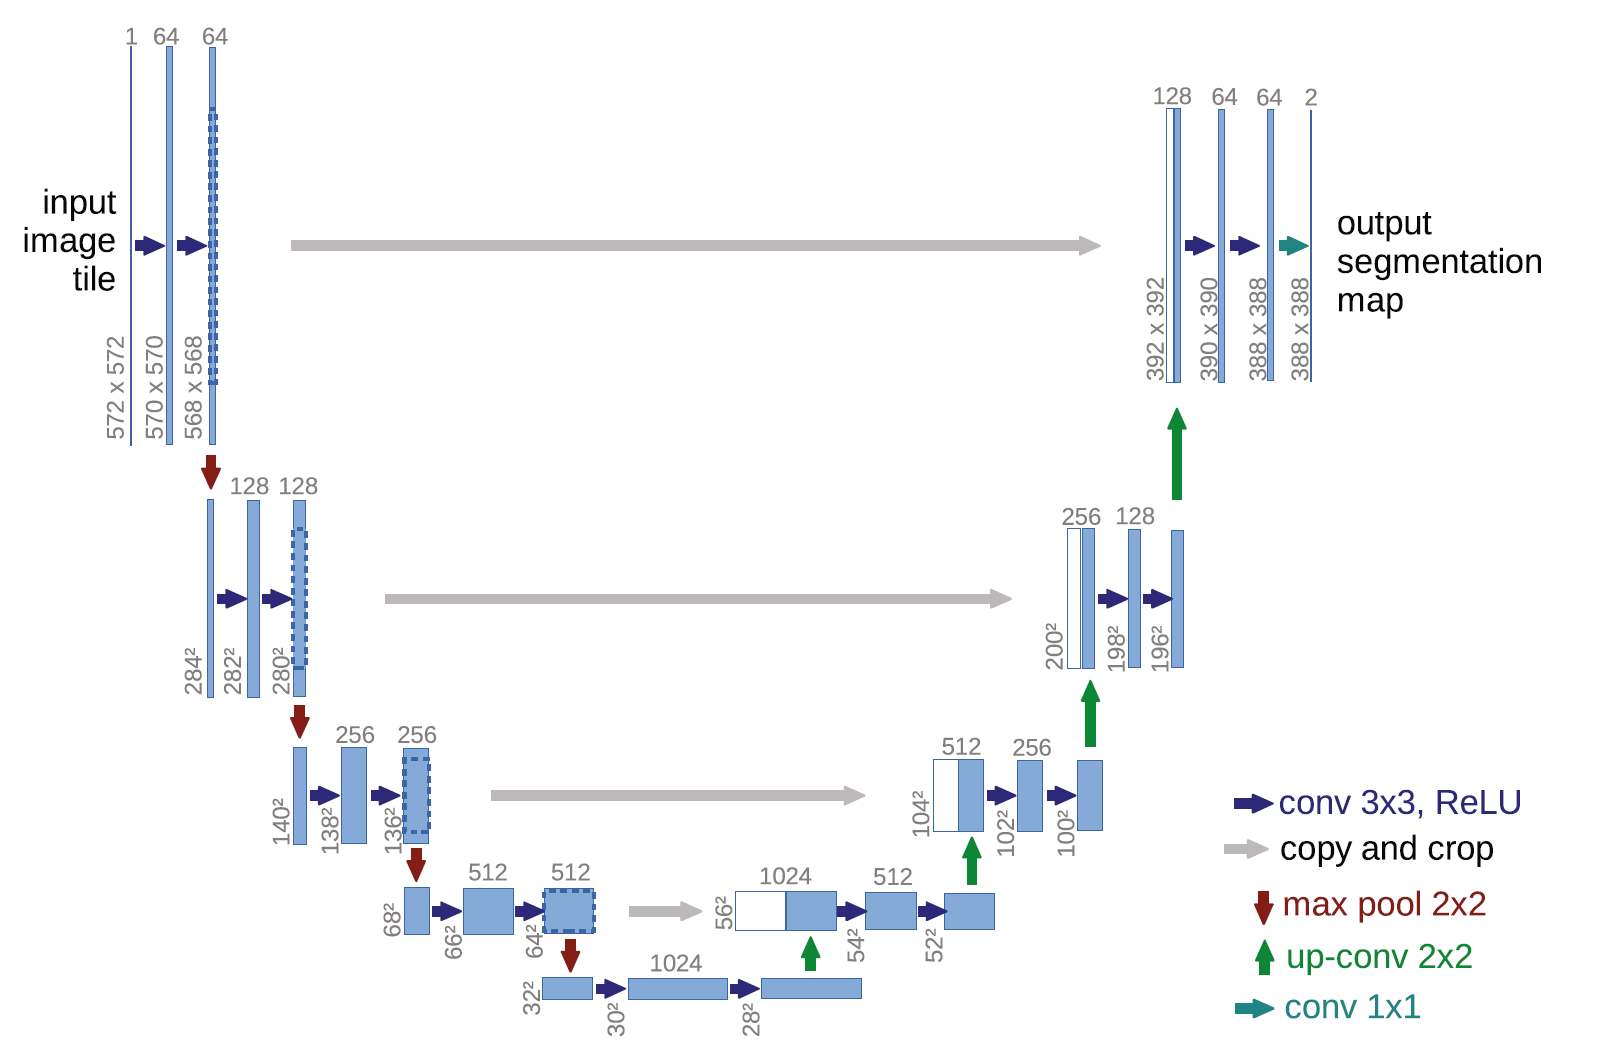
\includegraphics[width=.9\textwidth]{unet_aufbau.png}
	\caption{Aufbau eines U-Nets mit einem Encoder und Decoder Abschnitt für die Extrahierung von Merkmalen und die Wiederherstellung des Original Bildes mit der fertigen Segmentierung (Quelle: \cite{Ronneberger2015})}
	\label{fig:unet_aufbau}
\end{figure}
Die Architektur des Netzes besteht aus zwei Teilen, dem Downsampling Pfad, auch Encoder genannt, und dem Upsampling Pfad, der Decoder. Der Encoder ähnelt einem klassischen \ac{CNN} und besteht aus einer reihe von Convolutional und Max-Pooling Operationen, wobei es jedoch keine vollständig vernetzen Schichten gibt. 

Der Encoder wird verwenden, um die Feature-Maps aus dem Bild zu extrahieren. Bei jedem Schritt, den die Eingabe durch den Encoder macht, werden mehr Feature-Maps extrahiert und die räumliche Dimension des Bildes verringert. Die Ausgabe wird an die nächsthöhere Schicht weitergegeben, dies dient dazu möglichst viele Details auf verschiedenen Ebenen zu erhalten. Der Aufbau besteht dabei aus einer Reihe von zweifach Faltungen mit einem 3x3 Filter, auf die jeweils immer eine Max-Pooling Schicht mit einer Filtergröße von 2x2 und einer Schrittweite von 2 folgt. Bei jedem Encoder Schritt wird die Anzahl der Filter, bzw. Feature-Maps in den Faltungsschichten verdoppelt.

Im Decoder wird die komprimierte Eingabe wieder auf die ursprüngliche Bildgröße skaliert, auch ''Upsampling`` genannt. Dies geschieht durch eine Aneinanderreihung von Upsampling Schichten jeweils gefolgt von zweifach Faltungen und einer Aktivierungsfunktion. Nach jedem Upsampling der Feature-Maps folgt eine Faltung mit einem 2x2 Filter, welche die Anzahl der Feature-Maps jeweils halbiert. Hierbei findet zusätzlich eine Verkettung der Feature-Maps aus dem entsprechenden Encoder Abschnitt statt. Nach der 2x2-Faltung folgen jeweils immer zwei 3x3-Faltungen mit einer abschließenden ReLU Aktivierungsfunktion. Abschließend an den Decoder Abschnitt folgt noch eine Faltung mit einem 1x1 Filter, der die Features auf die gewünschte Anzahl von Klassen der Segmentierungsaufgabe abbildet. \cite[vgl.][]{Ronneberger2015}

\subsection{Hyperparameter}
Hyperparameter in neuronalen Netzwerken sind Parameter, deren Werte vor dem Training des Modells festgelegt und während des Trainings nicht angepasst werden bis auf gewisse Ausnahmen. Sie sind entscheidend für die Leistung des Modells und müssen sorgfältig ausgewählt werden. Die Auswahl der richtigen Hyperparameter ist oft eine Kunst und erfordert sowohl Erfahrung als auch experimentelles Ausprobieren. 

In der Praxis wird häufig eine Technik namens Hyperparametersuche oder -optimierung verwendet, bei der verschiedene Kombinationen von Hyperparametern systematisch ausprobiert werden, um diejenige zu finden, die die beste Leistung liefert. In diesem Abschnitt werden die wichtigsten Hyperparameter, die bei der Entwicklung des eines Deep Learning \glspl{Modell} relevant sind genauer beschrieben.

\paragraph{Lernrate} Die Lernrate ist ein entscheidender Hyperparameter in fast allen Optimierungsalgorithmen für Neuronale Netze. Sie bestimmt, wie stark die Gewichte im Netzwerk in jedem Schritt des Trainings angepasst werden. Eine zu hohe Lernrate kann dazu führen, dass das globale Minimum der Verlustfunktion übersprungen wird und das \gls{Modell} möglicherweise nicht konvergiert. Bei einer zu niedrigen Lernrate, wird der Fehler immer nur um sehr kleine Werte verringert, was zu einer langsamen Konvergenz führt. Es kann auch passieren, das der Fehler um einen Wert oszilliert und damit bei einer suboptimalen Lösung steckenbleibt. \cite[vgl.][]{Pfannstiel2022}

\paragraph{Batch Größe} Die Batch Größe bezieht sich auf die Anzahl der Trainingsbeispiele, die das Netzwerk gleichzeitig sieht, bevor es seine Gewichte aktualisiert. Eine größere Batch Größe kann zu stabileren Aktualisierungen der Gewichte führen, aber benötigt mehr Speicherplatz und verlangsamt das Training. Eine kleinere Batch Größe hingegen kann zu einem schnelleren, aber weniger stabilen Training führen. Übliche Größen für eine Batch reichen von 2, 8, 16 bis hin zu hunderten von Bildern in einer Batch. \cite[vgl.][]{Yu2020}

\paragraph{Anzahl der Epochen} Eine Epoche bezeichnet einen Durchlauf des gesamten Datensatzes während des Trainings. Die Anzahl der Epochen, für die das \gls{Modell} trainiert wird, beeinflusst, wie gut es Muster aus den Daten erlernen kann. Es ist wichtig eine geeignete Anzahl von Epochen auszuwählen, um einen optimalen Trainingsprozess zu erhalten. Bei einer zu niedrigen Anzahl an Epochen, hat das Netz nicht genügend Zeit, wichtige Muster zu lernen, wobei es zum Underfitting kommen kann. Ist die Anzahl der Epochen hingegen zu hoch, besteht die Gefahr, dass das Netz sich zu sehr an die Trainingsdaten anpasst und es zum Overfitting kommt. \cite[vgl.][]{Goodfellow2016}

\paragraph{Architektur spezifische Parameter} Im Kontext der U-Net Architektur gibt es auch spezifische Hyperparameter, die bei der Entwicklung des \glspl{Modell} berücksichtigt werden müssen, wie die Anzahl und Größe der Filter in den Faltungsschichten, sowie die Tiefe des Netzes und die Art der Aktivierungsfunktionen.


\subsection{Implementierung}
\label{subsec:Implementierung}
Die Implementierung des \gls{Modell}s für die Segmentierung der Gehirntumore erfolgt in Python mit PyTorch und basiert auf der U-Net Architektur, welche in \ref{sec:Modellarchitektur} erläutert wurde. Die Implementierung weicht in geringen Teilen von der originalen Architektur des U-Net ab. Die grobe Struktur des U-Net wurde weitestgehend übernommen, mit jeweils vier Down- und Upsampling Schichten. 

\subsubsection{Padding}
Aufgrund der Faltungen innerhalb des Netzes reduziert sich die Bildgröße, da keine Fülldaten verwendet werden. Um dem entgegenzuwirken, aus Gründen der besseren Implementierung, wird an jeden Rand des Bildes eine Bestimmte Anzahl von Pixeln hinzugefügt. Da die Bildgröße bekannt ist aufgrund der gegebenen Architektur (siehe Abschnitt \ref{paragraph:GrößenSkalierung}), kann für die Berechnung der Füllmenge $P$ die Formel \ref{eq:conv_size} verwendet werden. Die Bildgröße $W$ ist definiert durch ein vielfaches von $2^N$, wobei $N$ die Anzahl der Downsampling Schichten beschreibt. Im konkreten Fall ist $N=4$ und die Eingabegröße der Bilder ist 128x128 Pixel, was ein vielfaches von $2^N=2^4=16$ ist. Die Schrittweite $S$ und Filtergröße $F$ sind bereits durch den Aufbau des U-Net mit $S=1$ und $F=3$ gegeben. Daraus ergibt sich die Füllmenge mit Formel \ref{eq:conv_size}:
\begin{equation}
	P = \dfrac{W \times S - 1 - W + F}{2}
\end{equation}

\begin{equation}
	P = \dfrac{2^N \times 1 - 1 - 2^N + 3}{2}  = 1
\end{equation}
Durch das Beibehalten der Eingabegröße, ist die Implementierung aufgrund der einfachen Berechnung der Bildgröße für jede Schicht sehr von Vorteil. 

\subsubsection{Batch Normalisierung}
Die Batch Normalisierung ist eine Technik, die häufig beim Deep Learning verwendet wird, um das Training zu beschleunigen und die Stabilität des Netzwerks zu erhöhen. Das Vorgehen bei der Batch Normalisierung ist es, die Eingaben zu jeder Schicht zu normalisieren, indem die mittlere Aktivierung auf 0 und die Standardabweichung der Aktivierung auf 1 gesetzt wird.\\
Hierfür wird in der Regel der Mittelwert und die Standardabweichung für jedes Batch berechnet, daher auch der Name Batch Normalisierung. Es zeigte sich, dass durch Batch Normalisierung höhere Lernraten verwendet werden können und das Training im Allgemeinen schneller und effektiver verläuft. Zusätzlich wird die Stabilität des Netzwerks erhöht und die Notwendigkeit für sorgfältige Initialisierung der Modellparameter entfällt. Die Schicht wirkt außerdem teilweise als eine Art Dropout, bei welchem das Modell bestimmte Neuronen ``vergisst'' und neu initialisiert, um so ein Overfitting zu vermeiden.\cite[vgl.][]{Ioffe2015}
PyTorch stellt bereits eine Batch Normalisierungs Schicht zur Verfügung, die für die Normalisierung der Batches verwendet werden kann. Diese Schicht wird nach jeder Faltung und noch vor der Aktivierungsfunktion angewendet.

\subsection{Verlustfunktion}


\subsection{Probleme bei der Entwicklung}
% VRAM speicherplatz größe
% Schlechte Hardware
% CE Loss geht nicht

\subsection{Training}
